\section{Slacklining variations and categorization}\label{3_2_slacklineVariations}
Depending on the length, tension and/or height several slackline variations originated~\cite{MillerMauser2013-sl, Kleindl2011-bl, Thomann2017-ab}. Regarding the height one can differentiate between a \textit{lowline} (Figure \ref{fig:lowline}) and a \textit{highline} (Figure \ref{fig:highline}). Almost all lines match in the category lowline because it describes a height in which one can safely jump off the line. On a highline this is not possible. Here you have to make safety provisions like e.g. a seperate system in which the person can hook herself in this system above or under the regular line~\cite{Kleindl2011-bl}.
\begin{figure}[htb]
	\centering
	\begin{minipage}[t]{0.44\linewidth}
		\centering
		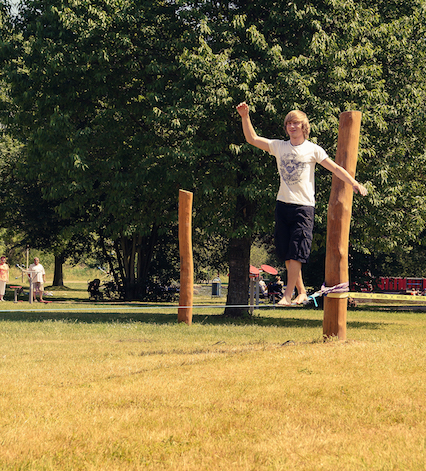
\includegraphics[width=0.94\linewidth]{Pictures/3_1_lowline}
		\subcaption{Common lowline}
		\label{fig:lowline}
	\end{minipage}
	\hfill
	\begin{minipage}[t]{0.44\linewidth}
		\centering
		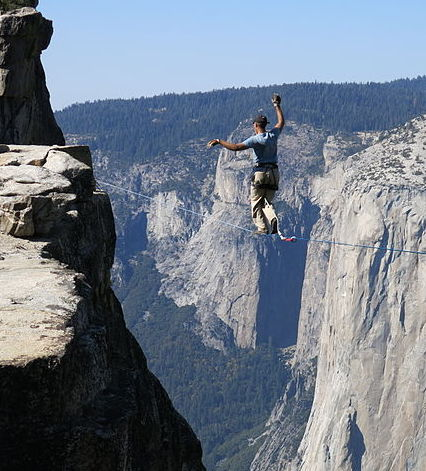
\includegraphics[width=0.94\linewidth]{Pictures/3_1_highline2}
		\subcaption{Highline between mountains~\cite{WikiSlacklining2017-lowline}}
		\label{fig:highline}
	\end{minipage}
	\caption{Main categories of slacklines}
	\label{fig:lowAndHighline}
\end{figure}

The following terms describe some fine granular variations as well as categorizations of the slackline in different application scenarios. They are not strict, which means they can differ in its scenario or can be combined each other. A common slackline is also named \textit{trickline} (Figure \ref{fig:trickline}). It is tensioned a bit loose in about the height of the knees and has a length up to 30 m. A \textit{jumpline} (Figure \ref{fig:jumpline}) is more tightly tensioned to simplify jumps on the line. It has a length of 8 - 14 m and is a bit higher than the trickline. With a \textit{rodeoline} the line is more slacked and and has the highest amplitude, like seen in figure \ref{fig:rodeoline}. It is a relatively short line with a length of 5 - 8 m and the fixation points are in about 2 m such that if a person stands in the mid of the line it is just about above the ground and can swing on it. Slacklines beyond 30 m are called \textit{longline} (Figure \ref{fig:longline}). The goal here is to walk as far as possible without falling off the line.

Beside these there exist some terms that describe a categorization or environment where a slackline can be applied. For example a \textit{waterline} is simply a line tensed over a pool, sea or a river like in figure \ref{fig:waterline}. \textit{Urbanlining} can be found in urban areas, where manmade buildings or structures are used to tense the line between, like in figure \ref{fig:urbanline}.
\begin{figure}[htb]
	\centering
	\begin{minipage}[t]{0.45\linewidth}
		\centering
		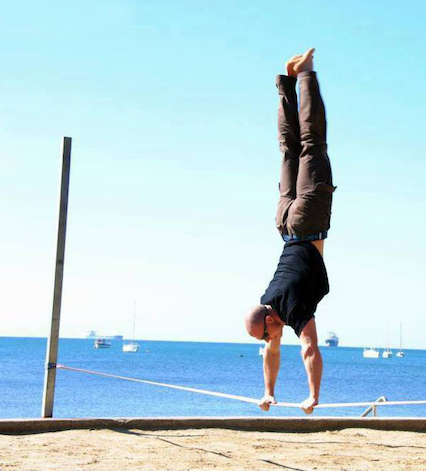
\includegraphics[width=1\linewidth]{Pictures/3_1_trickline}
		\subcaption{Handstand on a trickline~\cite{WikiSlacklining2017-trickline}}
		\label{fig:trickline}
	\end{minipage}
	\hfill
	\begin{minipage}[t]{0.45\linewidth}
		\centering
		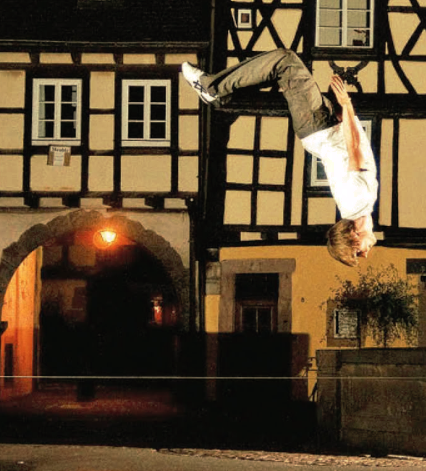
\includegraphics[width=1\linewidth]{Pictures/3_1_jumpline}
		\subcaption{Backflip on a jumpline~\cite{Kleindl2011-bl}}
		\label{fig:jumpline}
	\end{minipage}
	\hfill
	\begin{minipage}[t]{0.45\linewidth}
		\centering
		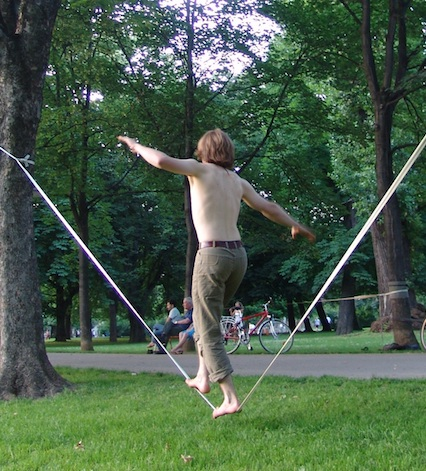
\includegraphics[width=1\linewidth]{Pictures/3_1_rodeoline}
		\subcaption{Rodeoline~\cite{WikiSlacklining2017-rodeoline}}
		\label{fig:rodeoline}
	\end{minipage}
	\hfill
	\begin{minipage}[t]{0.45\linewidth}
		\centering
		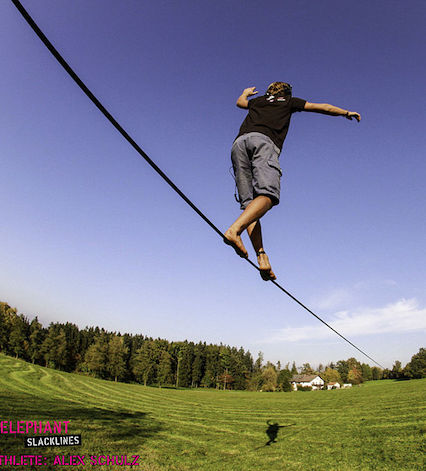
\includegraphics[width=1\linewidth]{Pictures/3_1_longline1}
		\subcaption{Longline~\cite{WikiSlacklining2017-longline}}
		\label{fig:longline}
	\end{minipage}
	\caption{Slackline variations}
	\label{fig:slacklineVariation}
\end{figure}
\clearpage
\begin{figure}[htb]
	\centering
	\begin{minipage}[t]{0.45\linewidth}
		\centering
		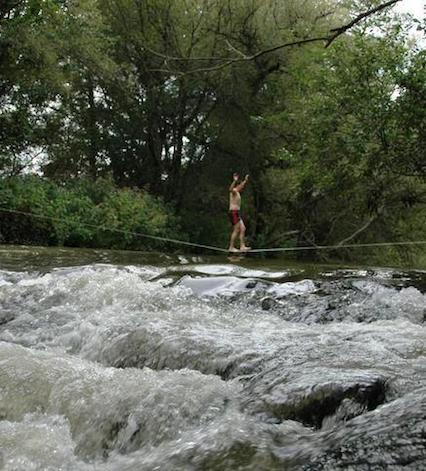
\includegraphics[width=1\linewidth]{Pictures/3_1_waterline}
		\subcaption{Waterlining over a river~\cite{WikiSlacklining2017-waterline}}
		\label{fig:waterline}
	\end{minipage}
	\hfill
	\begin{minipage}[t]{0.45\linewidth}
		\centering
		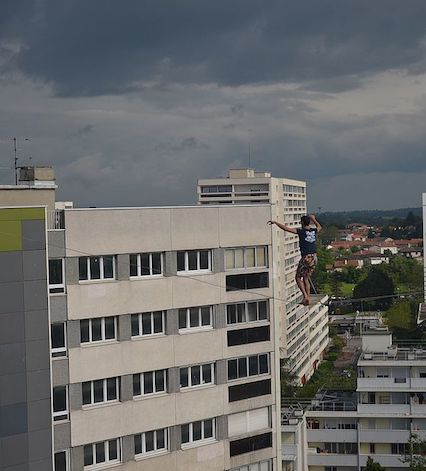
\includegraphics[width=1\linewidth]{Pictures/3_1_urbanline}
		\subcaption{Urbanlining in the city~\cite{WikiSlacklining2017-urbanline}}
		\label{fig:urbanline}
	\end{minipage}
	\caption{Categorization of slacklining}
	\label{fig:slacklineCategorization}
\end{figure}

The disadvantage of these lines is the inevitable usage of static fixation points. In the case of the slackline learning system this would result in a constraint of variability for developing, testing, and study purposes. For feasibility reasons and since the focus of the study lies mainly on beginners the slackline doesn't have to be very long. Therefore the choice felt on a mobile slackline device namely \textit{alpidex POWER-WAVE 2.0}\footnote{\url{http://www.alpidex.com/fitness/slacklines/slackline-gestell-in-2-laengen-power-wave-2-0-inklusive-slackline/a-10288/}}. It provides the needed mobility and independency due to its comparatively short length of three meters. The included slackline is tensed around brackets at both ends of the device. The middle rail is divided into two parts and needs to be put together. Hence it is possible to set it up indoors as well as move it in different positions with a minimum of effort~\ref{fig:3_2_mobileSlackline}.
\begin{figure}[htb]
	\centering
	\begin{minipage}[t]{1\linewidth}
		\centering
		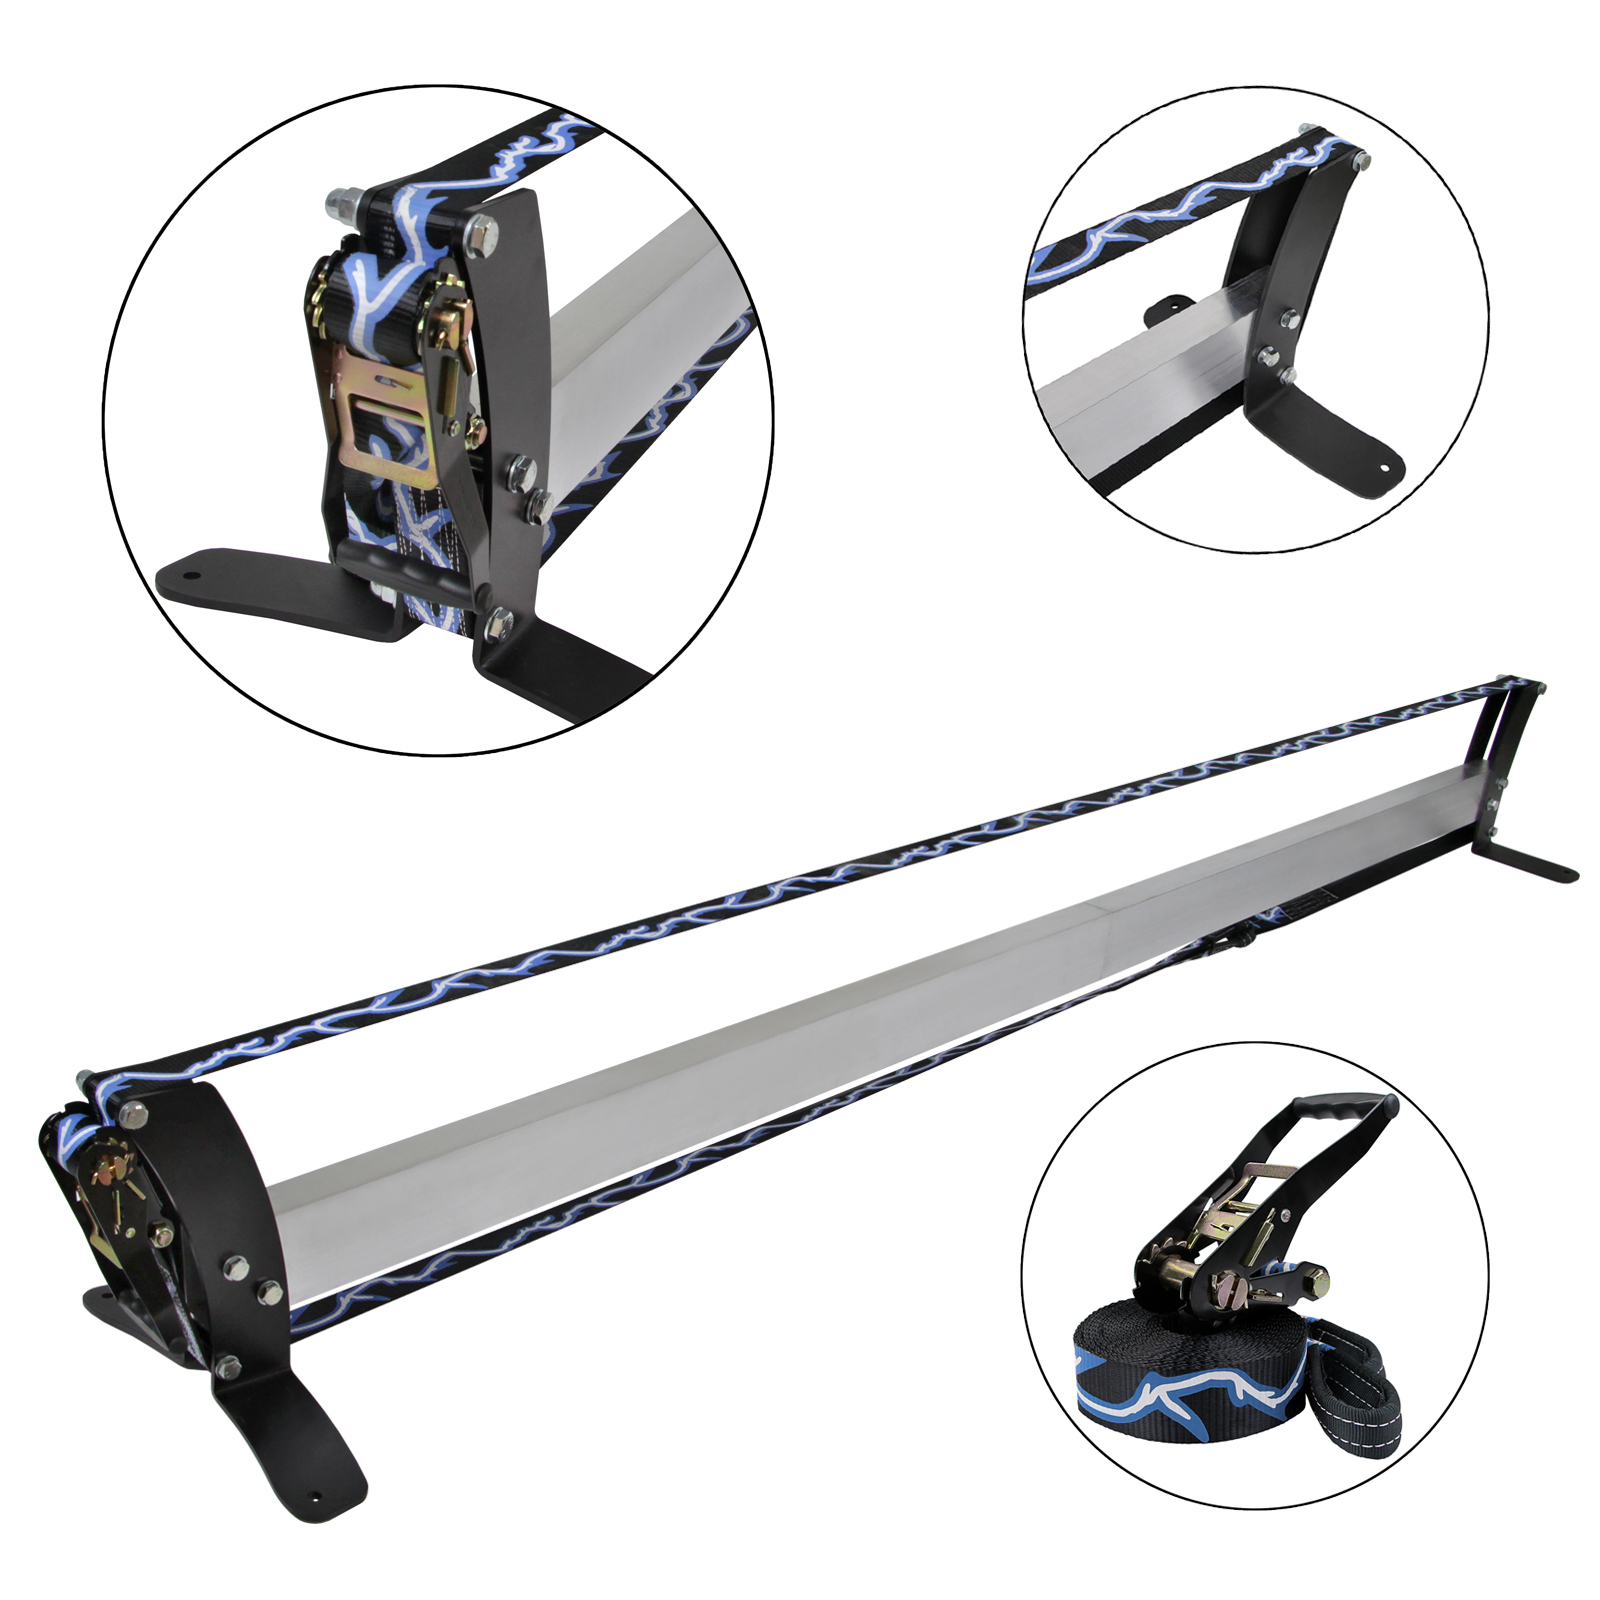
\includegraphics[width=0.44\linewidth]{Pictures/3_2_mobileSlackline}
		\caption{Mobile slackline \textit{alpidex POWER-WAVE 2.0}~\cite{alpidex2017-ms}}
		\label{fig:3_2_mobileSlackline}
	\end{minipage}
\end{figure}
